%!TEX TS-program = xelatex
%!TEX encoding = UTF-8 Unicode
\documentclass{article}
\usepackage[provide=*,dutch]{babel}

\usepackage{geometry}
\geometry{a4paper}
\usepackage[utf8]{inputenc}
\usepackage{enumitem}
\usepackage{hyperref}
\usepackage{graphicx}
\usepackage{tcolorbox}
\usepackage{float}
\usepackage{tabularx}
\hyphenation{wacht-tijd}
\hyphenation{wacht-tijden}
\setlength{\textheight}{240truemm}
% For better header handling
\usepackage{fancyhdr}
\pagestyle{fancy}
\fancyhf{}
\lhead{Ontwerpdocument Ingensche Veer}
\chead{IPASS}
\rhead{Vincent van Setten - 1734729}
\rfoot{Pagina \thepage}

% For colored text
\usepackage{xcolor}

\title{IPASS Plan van Aanpak}
\author{Vincent van Setten}

\begin{document}

\begin{titlepage}
    \begin{center}
        \vspace*{.6cm}
        \Huge
        \textbf{Ontwerpdocument }\\
        \vspace{0.2cm}
        \LARGE 
        \textbf{Ingensche Veer} \\
  
        \normalsize
  
  
        \vspace{1cm}
        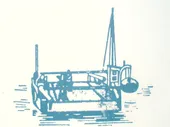
\includegraphics[width=0.7\textwidth]{images/iv.png}
        \vspace{1cm}
        \Large\\
        \textbf{In opdracht van}\\
        \large
        \textbf{University of Applied Sciences Utrecht} \\
        
\includegraphics[width=0.2\textwidth]{images/logouni.jpg}
  
        \vfill
      \end{center}
      \textbf{Datum:} \today \\
      \textbf{Versie:} 1.0 \\
      \textbf{Auteur:} Vincent van Setten \\
      \textbf{Studentnummer:} 1734729 \\
      \textbf{Klas:} V1C\\
  
  \end{titlepage}
  
  % ToC
  \tableofcontents
  \pagebreak 

  \section{Revisie Historie}
  \begin{table}[h]
      \centering
      \begin{tabular}{|c|c|c|p{5cm}|}
          \hline
          \textbf{Versie} & \textbf{Datum} & \textbf{Omschrijving}  \\
          \hline
          1.0  & 04-06-2024 & Eerste Versie \\
          \hline
  
      \end{tabular}
      \caption{Versiegeschiedenis}
  \end{table}
  \pagebreak

\section{Inleiding}
Tussen Ingen en Elst (Utrecht) ligt een veerpont. Deze gaat eigenlijk constant op en neer, zonder een vast tijdschema.
De veerpont is vrij groot en is voor zowel voetgangers, als auto's en fietsen. Er passen ongeveer 20 auto's op en een groot aantal fietsers en voetgangers.
De veerpont is relatief druk. Er worden dagelijks honderden mensen overgezet en is erg belangrijk voor de inwoners rondom Ingen en Elst. Het lastige met de drukte op de veerpont is dat het vaak in vlagen komt. De ene overtocht heeft slechts twee auto's en bij de volgende staan er zoveel dat niet alle auto's tegelijk over kunnen. Dit komt vooral omdat mensen niet weten wanneer de veerpont aankomt, waardoor veel mensen hem vaak net missen en vervolgens lang moeten wachten.
\par\smallskip 
Dat zorgt voor veel frustratie bij de klanten en veroorzaakt ook stress bij de schipper.
De kern van het probleem is dat klanten de aankomsttijd van de veerpont niet kunnen inschatten.
Een mogelijke oplossing voor dit probleem is de ontwikkeling van een webapplicatie die de huidige locatie van de veerpont weergeeft. Met deze applicatie kunnen klanten inschatten wanneer de veerpont aankomt, wat helpt bij het spreiden van de drukte en het verminderen van de wachttijden. Dit systeem zal gebruik maken van AIS-data om real-time informatie over de veerpont te bieden.
\par\smallskip 
De webapplicatie helpt ook met een ander probleem. Als het erg druk is, kan de baas van de veerpont extra hulp inschakelen. Momenteel gaat dat door puur te kijken op een bepaald moment hoe druk het is. 
Hiermee komt de hulp vaak net te laat, waardoor er een grote ophoping aan drukte ontstaat. Het is de bedoeling dat met de webapplicatie de schipper per overtocht kan aangeven hoe druk het is. Hiermee kan de baas zien wanneer er hulp nodig is, maar kan hiermee ook inschatten hoe druk het gaat worden op basis van historische data. 
\par\smallskip 
In dit ontwerpdocument wordt beschreven welke dingen er worden opgeleverd aan het eind van het IPASS project, hoe het project wordt aangepakt en er uiteindelijk uit gaat zien.
Ook worden de risico's en de planning van het project beschreven.


\section{Overzicht van het systeem}


\section{Use Cases}
\begin{figure}[h]
    \centering
    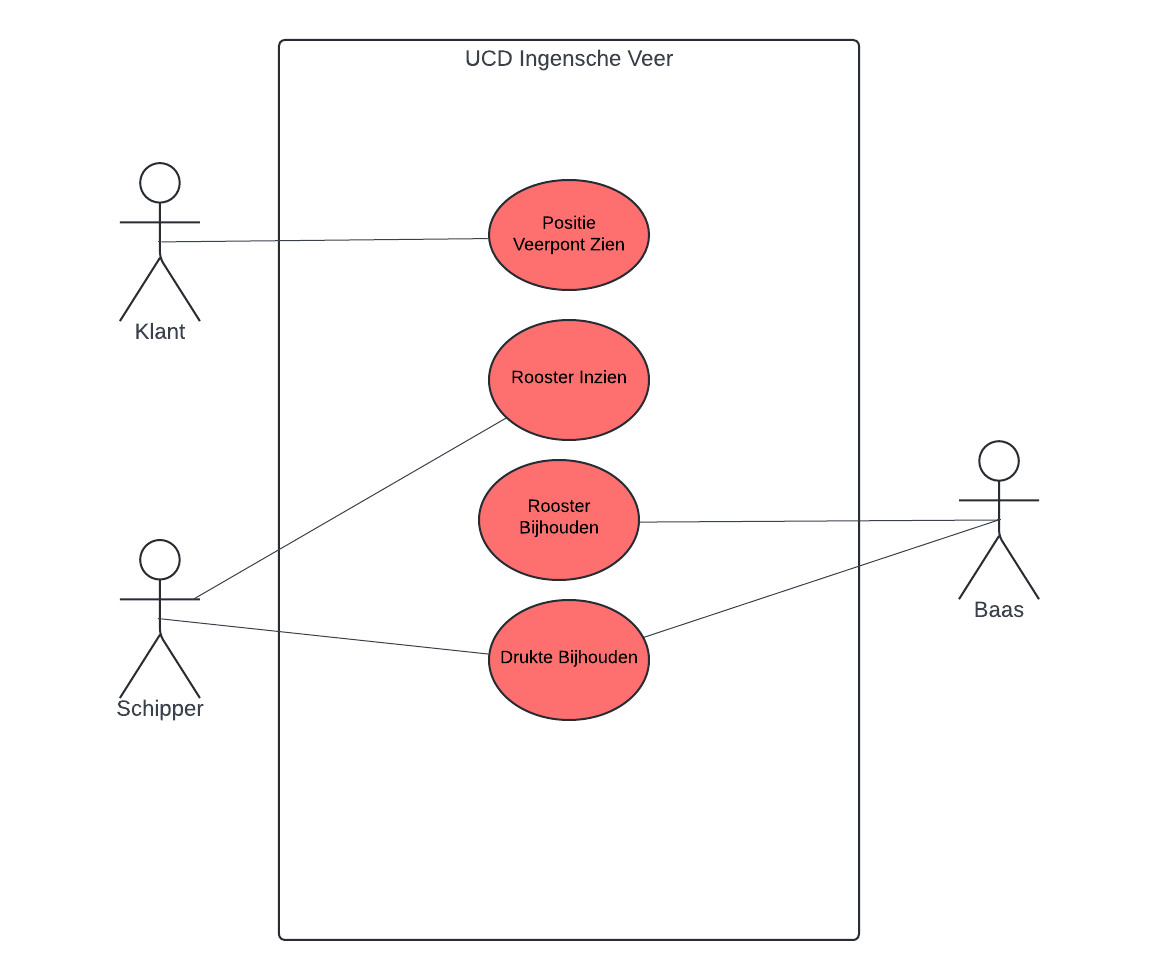
\includegraphics[width=0.7\textwidth]{images/iv_ucd_color.png}
    \caption{Use Case Diagram - Ingensche Veer}
    \label{fig:ucd}
\end{figure}
In het use case diagram in figuur \ref{fig:ucd} zie je de verschillende use cases. Deze zijn gekleurd naar het MoSCoW model. Rode use cases zijn Must haves, oranje use cases zijn Should haves, gele use cases zijn Could haves en groene use cases zijn Won't haves.

\subsection{Actoren}

\begin{table}[H]
    \centering
    \begin{tabularx}{\textwidth}{|l|X|}
        \hline
        \textbf{Actoren} & \textbf{Omschrijving}  \\
        \hline
        Baas & De baas is de eigenaar van de veerpont. \\
        \hline
        Klant  & De klant is de persoon die gebruik maakt van de veerpont. \\
        \hline
        Schipper & De schipper is de persoon die de veerpont vaart. \\
        \hline

    \end{tabularx}
    \caption{Actoren}
\end{table}

\subsection{Use case beschrijvingen en wireframes}
\subsubsection{UC01 - Bekijk locatie veerpont}
\begin{table}[H]
    \centering
    \begin{tabularx}{\textwidth}{|l|X|}
        \hline
        \textbf{ID:} UC01 & \textbf{Use Case Naam:} Bekijk locatie veerpont  \\
        \hline
        \textbf{Actoren:} & Klant \\
        \hline
        \textbf{Samenvatting:}  & De klant kan de actuele positie van de veerpont inzien op een kaart \\
        \hline 
        \textbf{Precondities:} & De veerpont stuurt AIS signalen en deze worden via de API ontvangen. \\
        \hline
        \textbf{Scenario:} & \begin{enumerate}
            \item De klant opent de webapplicatie
            \item Systeem haalt de actuele locatie van de veerpont op.
            \item Systeem toont de locatie van de veerpont op een kaart.
            \item De klant kan de locatie van de veerpont inzien.
        \end{enumerate} \\
        \hline 
        \textbf{Postcondities:} & nvt \\ 
        \hline

    \end{tabularx}
    \caption{Use Case Beschrijving UC01 - Bekijk locatie veerpont}
\end{table}

\begin{figure}[H]
    \centering
    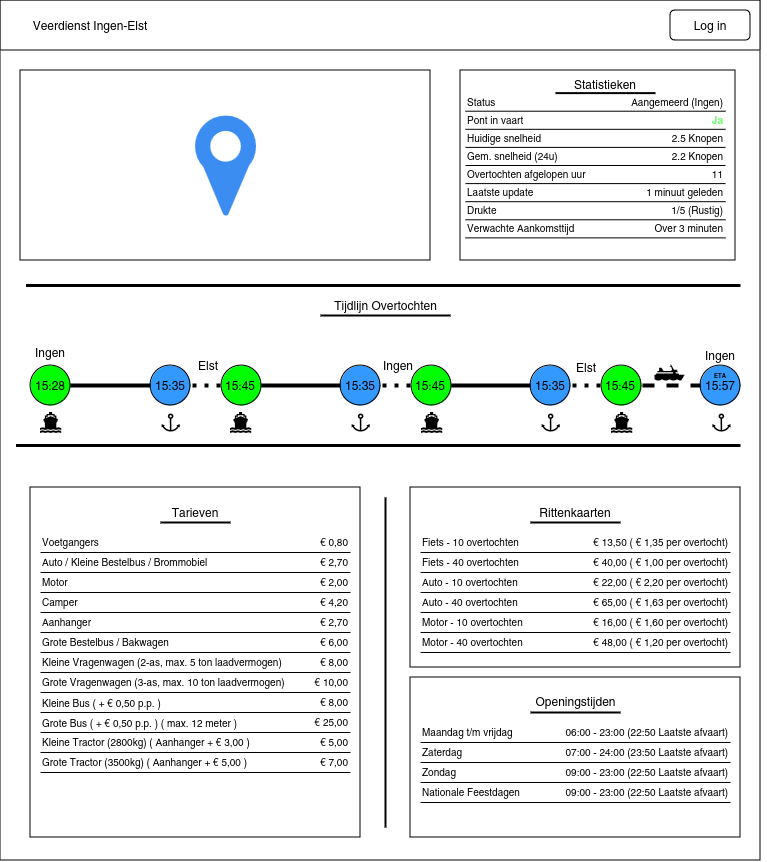
\includegraphics[width=0.8\textwidth]{images/wireframe_startpagina.png}
    \caption{Wireframe UC01 - Locatie veerpont bekijken}
    \label{fig:wf1}
\end{figure}

\section{Modellen}
\subsection{Domeinmodel}
\begin{figure}[H]
    \centering
    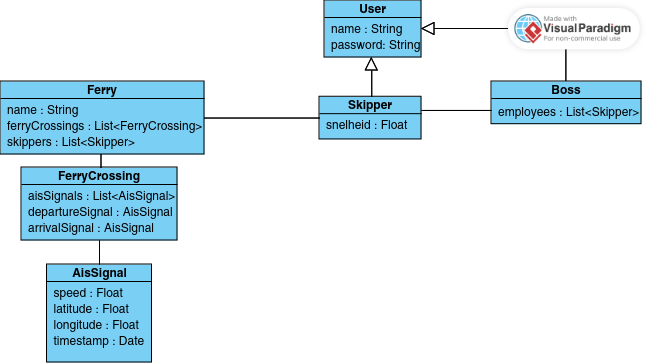
\includegraphics[width=0.8\textwidth]{images/ConceptueelKlassendiagram.png}
    \caption{Conceptueel Domeinmodel - Ingensche Veer}
    \label{fig:dm}
\end{figure}
In het domeinmodel in figuur \ref{fig:dm} zie je de Ferry klasse. Dit is de veerpont zelf. De veerpont houdt een lijst van overtochten bij, hier ferryCrossings genoemd. Een FerryCrossing houdt een lijst met AIS Signalen bij en daarnaast het signaal dat het vertek en de aankomst aangeeft. Het AIS signaal bevat de positie en tijd. Hiermee kan de positie van de veerpont worden laten zien.
De veerpont heeft ook een lijst met schippers. Een schipper heeft een snelheid, dat is hoeveel overtochten hij gemiddeld per uur maakt. Een schipper is, net als de baas, een gebruiker. De baas heeft zelf weer een lijst met schippers als werknemers.

\subsection{Business Rules}
Bij het domeinmodel in  figuur \ref{fig:dm} horen de volgende business rules:
\begin{enumerate}
    \item \textbf{Attribute Rule:} Een veerpont heeft minimaal een schippers.
    \item \textbf{Attribute Rule:} Een schipper heeft altijd maar één baas.
    \item \textbf{Entity Rule:} Elk AisSignaal heeft een snelheid, positie en tijd.
    \item \textbf{Entity Rule:} Elke gebruiker heeft een gebruikersnaam en wachtwoord.
    \item \textbf{Tuple Rule:} De datum van het verteksignaal is altijd kleiner dan de datum van het aankomstsignaal.
\end{enumerate} 

% \subsection{Datamodellen} alleeen als database
\section{Technologieen}
\begin{enumerate}
    \item UML
    \item Java 
    \item HTML 
    \item CSS 
    \item Javascript 
    \item Jax-RS(Rest)
    \item HTTP-Protocol 
\end{enumerate}

\section{Overdracht}
\section{Referenties}


\end{document}